\documentclass[12pt, titlepage]{article}

\usepackage{fullpage}
\usepackage[round]{natbib}
\usepackage{multirow}
\usepackage{booktabs}
\usepackage{tabularx}
\usepackage{graphicx}
\usepackage{float}
\usepackage{hyperref}
\hypersetup{
    colorlinks,
    citecolor=blue,
    filecolor=black,
    linkcolor=red,
    urlcolor=blue
}

%% Comments

\usepackage{color}

\newif\ifcomments\commentstrue %displays comments
%\newif\ifcomments\commentsfalse %so that comments do not display

\ifcomments
\newcommand{\authornote}[3]{\textcolor{#1}{[#3 ---#2]}}
\newcommand{\todo}[1]{\textcolor{red}{[TODO: #1]}}
\else
\newcommand{\authornote}[3]{}
\newcommand{\todo}[1]{}
\fi

\newcommand{\wss}[1]{\authornote{blue}{SS}{#1}} 
\newcommand{\plt}[1]{\authornote{magenta}{TPLT}{#1}} %For explanation of the template
\newcommand{\an}[1]{\authornote{cyan}{Author}{#1}}
%% Common Parts

\newcommand{\progname}{Software Engineering} % PUT YOUR PROGRAM NAME HERE
\newcommand{\authname}{Team \#12, Lower Earth Orbiters
\\ Diamond Ahuja
\\ Rishi Vaya
\\ Buu Ha
\\ Dhruv Cheemakurti
\\ Umang Rajkarnikar} % AUTHOR NAMES                  

\usepackage{hyperref}
    \hypersetup{colorlinks=true, linkcolor=blue, citecolor=blue, filecolor=blue,
                urlcolor=blue, unicode=false}
    \urlstyle{same}
                                


\newcounter{acnum}
\newcommand{\actheacnum}{AC\theacnum}
\newcommand{\acref}[1]{AC\ref{#1}}

\newcounter{ucnum}
\newcommand{\uctheucnum}{UC\theucnum}
\newcommand{\uref}[1]{UC\ref{#1}}

\newcounter{mnum}
\newcommand{\mthemnum}{M\themnum}
\newcommand{\mref}[1]{M\ref{#1}}

\begin{document}

\title{Module Guide for MCT }
\author{\authname}
\date{\today}

\maketitle

\pagenumbering{roman}

\section{Revision History}

\begin{tabularx}{\textwidth}{p{3cm}p{2cm}X}
\toprule {\bf Date} & {\bf Version} & {\bf Notes}\\
\midrule
Jan. 17, 2024 & 1.0 & Completed MG for MCT application\\
April 3, 2024 & 1.1 & Updated documentation to reflect current implementation of the application and updated MG based on feedback\\
\bottomrule
\end{tabularx}

\newpage

\section{Reference Material}

This section records information for easy reference.

\subsection{Abbreviations and Acronyms}

\renewcommand{\arraystretch}{1.2}
\begin{tabular}{l l} 
  \toprule		
  \textbf{symbol} & \textbf{description}\\
  \midrule 
  AC & Anticipated Change\\
  DAG & Directed Acyclic Graph \\
  M & Module \\
  MG & Module Guide \\
  OS & Operating System \\
  R & Requirement\\
  SC & Scientific Computing \\
  SRS & Software Requirements Specification\\
  UC & Unlikely Change \\
  FIFO & First In First Out \\
  MCT & Mission Control Terminal\\
  \bottomrule
\end{tabular}\\

\newpage

\tableofcontents

\listoftables

\listoffigures

\newpage

\pagenumbering{arabic}

\section{Introduction}

Decomposing a system into modules is a commonly accepted approach to developing
software.  A module is a work assignment for a programming
team.  We advocate a decomposition
based on the principle of information hiding.  This
principle supports design for change, because the ``secrets'' that each module
hides represent likely future changes.  Design for change is valuable in SC,
where modifications are frequent, especially during initial development as the
solution space is explored.  

Our design for the MCT application follows the rules layed out by the team, as follows:
\begin{itemize}
\item System details that are likely to change independently should be the
  secrets of separate modules.
\item Each data structure is implemented in only one module.
\item Any other program that requires information stored in a module's data
  structures must obtain it by calling access programs belonging to that module.
\end{itemize}

After completing the first stage of the design, the Software Requirements
Specification (SRS), the Module Guide (MG) is developed by Lower Earth Orbiters. The MG
specifies the modular structure of the system and is intended to allow both
designers and maintainers to easily identify the parts of the software.  The
potential readers of this document are as follows:

\begin{itemize}
\item New project members: This document can be a guide for a new project member
  to easily understand the overall structure and quickly find the
  relevant modules they are searching for.
\item Maintainers: The hierarchical structure of the module guide improves the
  maintainers' understanding when they need to make changes to the system. It is
  important for a maintainer to update the relevant sections of the document
  after changes have been made.
\item Designers: Once the module guide has been written, it can be used to
  check for consistency, feasibility, and flexibility. Designers can verify the
  system in various ways, such as consistency among modules, feasibility of the
  decomposition, and flexibility of the design.
\end{itemize}

The rest of the document is organized as follows. Section
\ref{SecChange} lists the anticipated and unlikely changes of the software
requirements. Section \ref{SecMH} summarizes the module decomposition that
was constructed according to the likely changes. Section \ref{SecConnection}
specifies the connections between the software requirements and the
modules. Section \ref{SecMD} gives a detailed description of the
modules. Section \ref{SecTM} includes two traceability matrices. One checks
the completeness of the design against the requirements provided in the SRS. The
other shows the relation between anticipated changes and the modules. Section
\ref{SecUse} describes the use relation between modules.

\section{Anticipated and Unlikely Changes} \label{SecChange}

This section lists possible changes to the system. According to the likeliness
of the change, the possible changes are classified into two
categories. Anticipated changes are listed in Section \ref{SecAchange}, and
unlikely changes are listed in Section \ref{SecUchange}.

\subsection{Anticipated Changes} \label{SecAchange}

Anticipated changes are the source of the information that is to be hidden
inside the modules. Ideally, changing one of the anticipated changes will only
require changing the one module that hides the associated decision. The approach
adapted here is called design for
change.

\begin{description}
\item[\refstepcounter{acnum} \actheacnum \label{acHardware}:] The specific TLE for satellites to track, per user.
\item[\refstepcounter{acnum} \actheacnum \label{acInput}:] The number of satellites to track, per user
\item[\refstepcounter{acnum} \actheacnum \label{acInput}:] The type of information requested by stakeholders 
\item[\refstepcounter{acnum} \actheacnum \label{acInput}:] The precision of measurement specification requested by stakeholders 
\item[\refstepcounter{acnum} \actheacnum \label{acInput}:] The ground station coordinate information 
\item[\refstepcounter{acnum} \actheacnum \label{acInput}:] The specific commands to be sent to satellites by operators and application administrators 
\end{description}

\subsection{Unlikely Changes} \label{SecUchange}

The module design should be as general as possible. However, a general system is
more complex. Sometimes this complexity is not necessary. Fixing some design
decisions at the system architecture stage can simplify the software design. If
these decision should later need to be changed, then many parts of the design
will potentially need to be modified. Hence, it is not intended that these
decisions will be changed.

\begin{description}
\item[\refstepcounter{ucnum} \uctheucnum \label{ucIO}:] Server on which the application in hosted
\item[\refstepcounter{ucnum} \uctheucnum \label{ucIO}:] Format of satellite data input 
\item[\refstepcounter{ucnum} \uctheucnum \label{ucIO}:] Format of TLE data for tracking 
\item[\refstepcounter{ucnum} \uctheucnum \label{ucIO}:] Encoding scheme of command sequences to be sent to a satellite 
\item[\refstepcounter{ucnum} \uctheucnum \label{ucIO}:] Database technology being used to persist command sequences and log outputs 
\end{description}

\section{Module Hierarchy} \label{SecMH}

This section provides an overview of the module design. Modules are summarized
in a hierarchy decomposed by secrets in Table \ref{TblMH}. The modules listed
below, which are leaves in the hierarchy tree, are the modules that will
actually be implemented.

\begin{description}
\item [\refstepcounter{mnum} \mthemnum \label{mHH}:] Hardware-Hiding Module
\item ...
\end{description}


\begin{table}[h!]
\centering
\begin{tabular}{p{0.3\textwidth} p{0.6\textwidth}}
\toprule
\textbf{Level 1} & \textbf{Level 2}\\
\midrule

{Hardware-Hiding Module} & N/A ~ \\
\midrule

\multirow{7}{0.3\textwidth}{Behaviour-Hiding Module} & Satellite Module\\
& Schedule Module\\
& User Module\\
& Log Module\\
& Database Module\\
& Authentication Module\\
& BackendService Module \\
\midrule

\multirow{1}{0.3\textwidth}{Software Decision Module} & SatelliteQueue Module \\
\midrule

\end{tabular}
\caption{Module Hierarchy}
\label{TblMH}
\end{table}

\section{Connection Between Requirements and Design} \label{SecConnection}

The design of the system is intended to satisfy the requirements developed in
the SRS. In this stage, the system is decomposed into modules. The connection
between requirements and modules is listed in Table~\ref{TblRT}.

\subsection{Modules}

\subsubsection{Satellite Module}

The Satellite module is responsible for all information related to a satellite, including calculating positional data, future overpasses, and generating polar plot data.

\subsubsection{Schedule Module}

The Schedule module is responsible for all logic pertaining to storing, updating, and executing command sequence(s) for a satellite target.

\subsubsection{User Module}

The User module is responsible for storing information about users in the MCT application. This includes creating new users and updating information for existing users.

\subsubsection{SatelliteQueue Module}

The SatelliteQueue module implements the queue data structure to store commands scheduled for execution in the upcoming overpass.

\subsubsection{Log Module}

The Log module implements logging functionality from the ground server.

\subsubsection{Authentication Module}

This module will employ the user's email and password for authentication purposes and to fetch their complete information, a prerequisite for accessing the satellite and scheduling data.

\subsubsection{Database Module}

This module will utilize multiple data structures to store, collect and return data. It will also enable users to view and edit stored data.

\subsubsection{BackendService Module}

It's responsible for initializing the backend processes of the application.  
 
\section{Module Decomposition} \label{SecMD}

Modules are decomposed according to the principle of ``information hiding''. The \emph{Secrets} field in a module
decomposition is a brief statement of the design decision hidden by the
module. The \emph{Services} field specifies \emph{what} the module will do
without documenting \emph{how} to do it. For each module, a suggestion for the
implementing software is given under the \emph{Implemented By} title. If the
entry is \emph{OS}, this means that the module is provided by the operating
system or by standard programming language libraries.  \emph{MCT} means the
module will be implemented by the MCT software.

Only the leaf modules in the hierarchy have to be implemented. If a dash
(\emph{--}) is shown, this means that the module is not a leaf and will not have
to be implemented.

\subsection{Hardware Hiding Modules (\mref{mHH})}

\begin{description}
\item N/A
\end{description}

\subsection{Behaviour-Hiding Module}


 
\begin{description}
\item[Secrets:]The contents of the required behaviours.
\item[Services:]Includes programs that provide externally visible behaviour of
  the system as specified in the software requirements specification (SRS)
  documents. This module serves as a communication layer between the
  hardware-hiding module and the software decision module. The programs in this
  module will need to change if there are changes in the SRS.
\item[Implemented By:] --
\end{description}

\subsubsection{Satellite Module}

\begin{description}
\item[Secrets:]Overpass dates, satellite name and intl code.
\item[Services:]Fetch future overpasses, satellite telemetry information and manage (add, update, delete) records of satellite systems.
\item[Implemented By:] MCT
\item[Type of Module:] Abstract Object
\end{description}

\subsubsection{Schedule Module }

\begin{description}
\item[Secrets:] Command sequences to execute for a satellite's scheduled overpass.
\item[Services:]Manage (add, update, delete) records of scheduled command sequences for a satellite system.
\item[Implemented By:] MCT
\item[Type of Module:] Abstract Object
\end{description}

\subsubsection{User Module }

\begin{description}
\item[Secrets:] User email and role.
\item[Services:] Manages (reads, creates, updates) user records.
\item[Implemented By:] MCT
\item[Type of Module:] Abstract Object
\end{description}

\subsubsection{Authentication Module }

\begin{description}
\item[Secrets:] User email and password.
\item[Services:] Registers and signs users to the MCT application.
\item[Implemented By:] Auth0
\item[Type of Module:] Library
\end{description}

\subsubsection{Database Module }

\begin{description}
\item[Secrets:] Records to store, update and remove from the database.
\item[Services:] Stores data and provides read and write access to the data store.
\item[Implemented By:] MongoDB
\item[Type of Module:] Library
\end{description}

\subsubsection{Log Module }

\begin{description}
\item[Secrets:] SatelliteId to find logs for a particular satellite.
\item[Services:] Gets logs for all executed commands for a specific satellite.
\item[Implemented By:] MCT
\item[Type of Module:] Abstract Object
\end{description}

\subsection{Software Decision Module}

\subsubsection{SatelliteQueue Module}

\begin{description}
\item[Secrets:] An array to manage scheduled command sequences for the next overpass in a FIFO order. This ensures that the queued commands will always be up to date.
\item[Services:] Queue data structure to store commands scheduled for execution in the upcoming overpass.
\item[Implemented By:] SatelliteQueue Module
\end{description}



\section{Traceability Matrix} \label{SecTM}

This section shows two traceability matrices: between the modules and the
requirements and between the modules and the anticipated changes.

% the table should use mref, the requirements should be named, use something
% like fref

 
\begin{table}[H]
\centering
\begin{tabular}{|c|c|c|} \hline 
% \begin{tabular}{p{0.2\textwidth} p{0.6\textwidth}}
\toprule
\textbf{Req.} & \textbf{Modules} & \textbf{Module Numbers}\\
\midrule

REQ-MCT-001 & BackendService & 6.1.8  \\ 

REQ-MCT-002 & User & 7.2.3 \\ 

REQ-MCT-003 & Authentication, User & 7.2.4, 7.2.3 \\ 

REQ-MCT-004 & Schedule & 7.2.2 \\ 

REQ-MCT-005 & Schedule & 7.2.2 \\ 

REQ-MCT-006 & Satellite & 7.2.1 \\ 

REQ-MCT-007 & Satellite, Schedule & 7.2.1, 7.2.2 \\ 

REQ-MCT-008 & Satellite, Log & 7.2.1, 7.2.6 \\ 

REQ-MCT-009 & Schedule & 7.2.2 \\ 

REQ-MCT-010 & Schedule & 7.2.2 \\ 

REQ-MCT-011 & Schedule & 7.2.2 \\ 

REQ-MCT-012 & Schedule & 7.2.2 \\ 

REQ-MCT-013 & Schedule & 7.2.2 \\ 

REQ-MCT-014 & Schedule & 7.2.2 \\ 

REQ-MCT-015 & User & 7.2.3 \\ 

REQ-MCT-016 & User & 7.2.3 \\ 

REQ-MCT-017 & User & 7.2.3 \\ 

REQ-MCT-018 & User, Schedule & 7.2.3 7.2.2 \\ 

REQ-MCT-019 & Schedule & 7.2.2 \\ 

REQ-MCT-020 & Schedule & 7.2.2 \\ 

REQ-MCT-021 & Schedule & 7.2.2 \\ 

REQ-MCT-022 & Satellite & 7.2.1 \\ 

REQ-MCT-023 & Satellite & 7.2.1 \\ 

REQ-MCT-024 & Satellite & 7.2.1 \\ 

REQ-MCT-025 & Satellite & 7.2.1 \\ 

REQ-MCT-026 & Satellite & 7.2.1 \\ 

REQ-MCT-027 & Satellite, Schedule, SatelliteQueue & 7.2.1, 7.2.2 \\ 

REQ-MCT-028 & Satellite, Schedule, SatelliteQueue & 7.2.1, 7.2.2 \\ 

OPT-MCT-001 & Schedule & 7.2.2 \\ 

OPT-MCT-002 & Schedule & 7.2.2 \\ 

OPT-MCT-003 & Schedule & 7.2.2 \\ 

OPT-MCT-004 & Schedule & 7.2.2 \\ 

OPT-MCT-005 & Schedule & 7.2.2 \\ 

OPT-MCT-006 & Schedule & 7.2.2 \\ 

OPT-MCT-007 & Schedule & 7.2.2 \\ 

OPT-MCT-008 & BackendService & 6.1.8 \\

\bottomrule
\end{tabular}
\caption{Trace Between Requirements and Modules}
\label{TblRT}
\end{table}

\begin{table}[H]
\centering
\begin{tabular}{|c|c|c|} \hline 
\toprule
Anticipated Change
& Modules & Module Numbers
\\
\midrule

AC1
& Satellite & 7.2.1
\\
AC2
& Satellite & 7.2.1
\\
AC3
& Satellite & 7.2.1
\\
AC4
& Satellite & 7.2.1
\\
AC5
& Satellite & 7.2.1
\\
AC6
& Satellite, Schedule & 7.2.1, 7.2.2
\\
\bottomrule
\end{tabular}
\caption{Trace Between Anticipated Changes and Modules}
\label{TblACT}
\end{table}

\section{Use Hierarchy Between Modules} \label{SecUse}

The Log module is one of the basic modules in the hierarchy. Both Satellite Queue and Database modules use it for logging. The User module uses the Database module too for managing user-related data. The Backend Service is the orchestrator of the system, and some of the key components employed by the Backend Service to assume its roles include the User and Authentication modules and the Satellite Queue with the Schedule, all to manage the satellite data and operations. This implies a hierarchy situation where every higher-level module depends on the functioning of lower ones, thereby, allowing systematic testing of the system architecture without having circle dependencies.



\begin{figure}[H]
\centering
\begin{figure}
    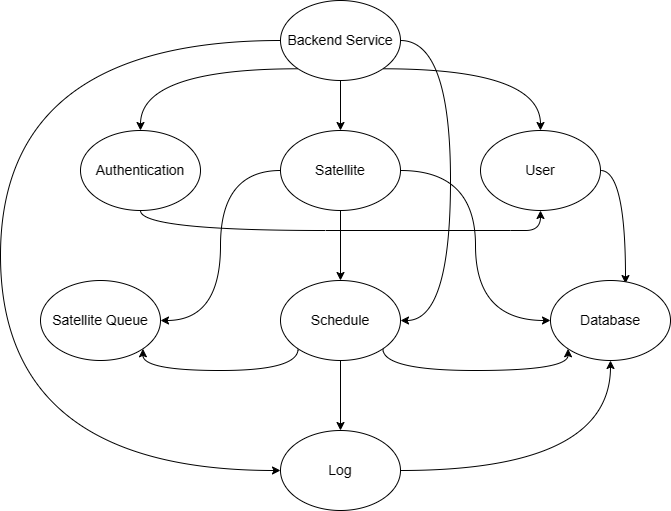
\includegraphics[width=1\linewidth]{hierarchy_dag.png}
    \caption{DAG diagram depicting the hierarchy between modules}
    \label{Use hierarchy among modules}
\end{figure}
\label{FigUH}
\end{figure}

\section{Timeline}

The deadlines in our project's timeline are planned to match the main goals we aim to achieve in each stage. We've split the work into parts, each with its own deadline, so we can work on different things at the same time and make sure everything comes together smoothly. For example, we're finishing the User module early because it's important for setting up who can do what in the system. Getting the Authentication module done early is also key because it makes sure that only the right people can access the system while we keep building it. The set deadlines help us keep track of our progress. This way, we can make sure we finish the whole project on time without rushing and making mistakes. In short, our timeline helps us stay organized and work efficiently so that we can complete our project successfully and on time.
\\
\begin{center}
    \begin{table}
    \centering
    \begin{tabular}{p{0.6\textwidth} p{0.2\textwidth} p{0.2\textwidth}}

    % \begin{tabular}{|c|c|c|} \hline 
         \textbf{Module and Description}&  \textbf{People Responsible}& \textbf{Deadline}\\ \hline 
         Satellite (7.2.1) - Should implement future overpass, satellite information and record updating functionalities. Should add test cases for all the endpoints created&  Quinn& Jan 31, 2024\\ \hline 
         Schedule (7.2.2) - should create the endpoints required for adding commands to schedules and testing them&  Quinn, Umang, Rishi& Jan 31, 2024\\ \hline 
         User (7.2.3) - should create endpoints for creating, updating and permissions for users. Should add test cases for all the endpoints created&  Dhruv& Jan 25, 2024\\ \hline 
         SatelliteQueue (6.1.4) - Should add the functionality to execute schedules in the satellite queue based on the overpass times.&  Umang, Rishi& Jan 31, 2024\\ \hline 
         Log (7.2.6) - should create endpoint to receive logs for all commands and make the frontend page.&  Quinn& Jan 20, 2024\\ \hline 
         Authentication (7.2.4) - should create functionality to authenticate a user using auth0&  Diamond& Jan 25, 2024\\ \hline 
         Database (6.1.7) - should create all the schemas for users, satellites, commands, schedules and logs.&  Umang, Rishi& Jan 31, 2024\\ \hline 
         % BackendService (6.1.8)&  Diamond, Dhruv& Jan 31, 2024\\ \hline
    \end{tabular}
    \caption{Table for the timeline of the module}
    \label{tab:my_label}
\end{table}
\end{center}

%\section*{References}

\end{document}